%% Artyom Voronin
%%  __     _ _                   
%% / _| __| (_)  _ __  _ __ ___  
%%| |_ / _` | | | '_ \| '_ ` _ \ 
%%|  _| (_| | | | |_) | | | | | |
%%|_|  \__,_|_| | .__/|_| |_| |_|
%%              |_|              
%% Brno, 2021

\chapter{Theoretical Survey}\label{ch:teor_surv}

This chapter contains a short introduction to the main goals and problems
presented in fault detection and analysis and predictive maintenance
techniques. A brief review of methodologies used in these fields and
general approaches.

Section digital twin presents scenarios where a simulation model is used in
predictive maintenance. 


% -----------------------------------------------------------------------------
% 
% -----------------------------------------------------------------------------

\section{Problem Definition}

% XXX FaultDetectionMethods-ALiteratureSurvay.pdf

In practice many types of machinery require some calibration and monitoring
for adequate working. An anomaly or fault detection in time can prevent
machinery from damage that causes loss of money due to non-working or
destroyed equipment.  Predicting where the fault appears reduces the cost
of diagnosis and replacement operations. The possibility of estimating the
remaining useful life allows to optimize a maintenance process and reduce
maintenance costs.


Smart manufacturing, the combination of sensors, the possibility of
preprocessing and extracting useful information from measurements and
decision algorithms based on this information, allows increasing production
efficiency and significantly reducing maintenance operations.



\paragraph{Types of Maintenance} There are three main types of maintenances
\ref{fig:maintenance}. Each following type of maintenance requires
increasing complexity of monitoring
and decision algorithms:

\begin{itemize}
    \item Reactive maintenance, where maintenance coming after the life of
        the system is excess.
    \item Preventive maintenance is driven item by
        schedules that may keep the system safe but not optimal from an
        efficiency/cost perspective. 
    \item Predictive maintenance is an
        effort to optimize a maintenance strategy.
\end{itemize}

\begin{figure}[h!]
    \centering
    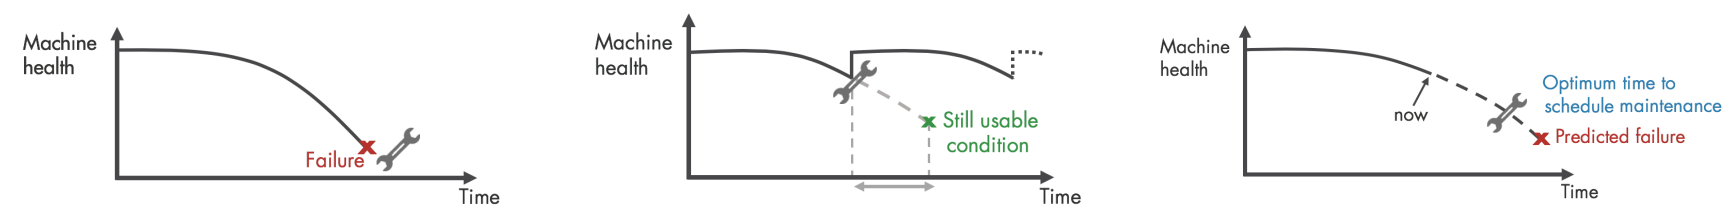
\includegraphics[width=1.1\textwidth]{maintenance.png}
    \caption{Reactive, preventive and predictive types of maintenance}
    \label{fig:maintenance}
\end{figure}


\paragraph{Fault Types} A fault is not an acceptable deviation of at least one
characteristic or parameter of the system from the standard condition.
There are different faults by their sources. 
\begin{itemize}
    \item Plant faults appear in system
        behavior and cause manufacturing performance.
    \item Component fault
    \item Sensor faults occurred in the sensor during measurements.
    \item Combination of faults
\end{itemize}
In many cases, faults lead to a system failure and
the system is no longer able to perform required functions.
There may also be a malfunction after which the system returns to normal
operation. 

Faults can be classified by the location where they appear, by a fault
form, or based on the form in which the fault is added to the system.


% -----------------------------------------------------------------------------
% 
% -----------------------------------------------------------------------------

\section{Fault Detection and Analysis (FDA)}

Fault Detection and Analysis, FDA (Fault Detection and Isolation, FDI) is a
subfield of control engineering focused on detecting the fault and
identifying where this fault is located. 
The main goals of FDI are
\begin{itemize}
    \item Fault detection, detect anomalies in real-time
    \item Fault isolation, find the root cause
    \item Fault identification, estimation of the magnitude, type, or nature of
        the fault 
\end{itemize}

Several methods are partly overlapped but divided into two main
categories. 

\paragraph{Signal-Based methods} Signal-Based methods (SB), explore measured
data and extract useful information in the form of features
\ref{fig:signal_based}. The following methods belong to the SB approach: 

\begin{itemize}
    \item Limit and trend checking
    \item Spectral analysis
    \item Data analysis (PCA)
    \item Pattern recognition
\end{itemize}

\begin{figure}[h!]
    \centering
    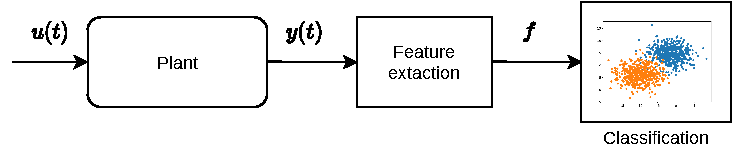
\includegraphics[width=0.7\textwidth]{signal_based.pdf}
    \caption{Signal-Based Method}
    \label{fig:signal_based}
\end{figure}


\paragraph{Model-Based methods} Model-Based methods exploit models identified
from real-life systems \ref{fig:model_based}. The model-based approach is
suitable when it is difficult to gain useful information using only
measured signals. If the system structure is known, it is possible to
extract features such as state variables or some system parameters.
Another option is to compare real system behavior with nominal healthy
model and use residuals as inputs to decision algorithms.
Typical model-based techniques include

\begin{itemize}
    \item Residual estimation (compare measurements with "healthy" model)
    \item Polynomial coefficients
    \item State variables estimated using state observers
    \item Parameter estimation
\end{itemize}

\begin{figure}[h!]
    \centering
    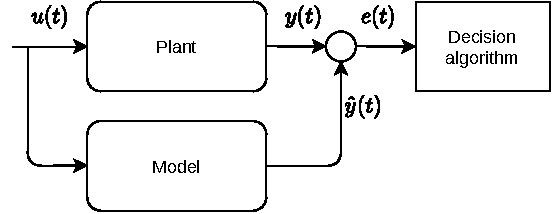
\includegraphics[width=0.5\textwidth]{model_based.pdf}
    \caption{Model-Based Method}
    \label{fig:model_based}
\end{figure}


Automated fault detection depends on input from sensors and postprocessing
algorithms. In many manufacturing applications, sensor failures are the
most common equipment failure.


The result of FDI is the detection and identification of faults that occur
during the operation of the device. Subsequently, predicted faults are
processed using fault tolerance and predictive maintenance algorithms.

\textbf{Fault Tolerance}: Provide the system with the hardware architecture
and software mechanisms that will allow, if possible, to achieve a given
objective in normal operation and given fault situations.

%\subsection{Condition Monitoring}
%Answer to question:"How does system operate now?"
%CM gives Diagnostic methods that provides alarm or warning, but not
%prognostic forecast about the future behavior (Not RUL).
%
%But collected Condition Monitoring information can give information about
%system degradation.
%
%
%There is a optimization between technical and financial possibilities in a
%specific situation.
%
%FMECA (Failure Mode, Effect and Criticality Analysis) \\
%FTA (Fault Tree Analysis) \\
%RCA (Root Cause Analysis) \\


% -----------------------------------------------------------------------------
% 
% -----------------------------------------------------------------------------


\section{Predictive maintenance (PdM)}
\textbf{Predictive maintenance (PdM)} is cost-effective maintenance strategy that
predicts time to failure and warns of an anticipated location where this
could occur.

\subsection{Goals}
The are two main goals of Predictive maintenance, RUL (remaining useful
life) estimation and identification where the future failure can appear, or what is
the reason of decreasing RUL. 
As a result of PdM is RUL representing of number cycles, days, or some time
period before fault occurred. And probability where this fault can appear.

\subsection{Overview of the PdM development sequence}

\begin{figure}[h!]
    \centering
    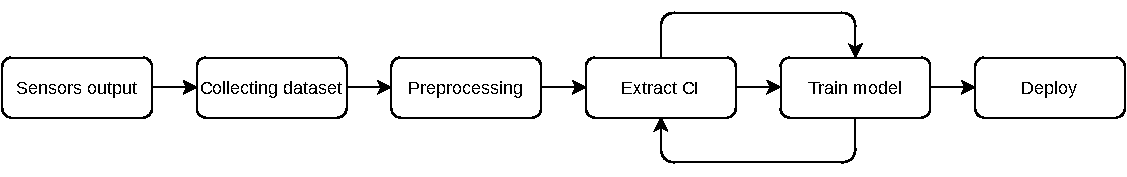
\includegraphics[width=1\textwidth]{pdm_deploy_sequence.pdf}
    \caption{Predictive maintenance development sequence}
    \label{fig:pdm_dev_seq}
\end{figure}

Figure \ref{fig:pdm_dev_seq} represents the recommended PdM development
workflow.  The development of predictive maintenance algorithms starts with
raw measured signals from sensors. For further working with data, it's an
excellent manner to combine measurements to a dataset with a logical
structure of elements. In this thesis, a common data ensemble structure was
used. Each measurement has its data file with all measured signals at a
particular time. 

If collected data require some preprocessing techniques as data cleaning,
smoothing or filter the signal, detrend, normalizing, etc., it can be done
at this step. 

The next step is to extract condition indicators using predictive
maintenance methods described in \ref{sec:ci}. Figure out the best
combination of CI to train the classification model. As long as the optimal
solution not find, try to figure out the best combination of CI described
in \ref{sec:ci_ranking} and train different classification models
iteratively.  After the efficient solution is found, deploy the algorithm
to work recursively with the study-case system.


\subsection{Condition Indicators}\label{sec:ci}
In the prediction maintenance field, features extracted from measured
signals are called \textbf{Condition Indicators, CI}.

Condition Indicators represent some system behavior and hide information
about system operation conditions.  Generally, CI is represented by three
main domains. There is a time domain, frequency domain, time-frequency
domain. But in fact, CI can be any system parameter or value corresponding
with the system's current condition.

The methods of extracting condition indicators from the signal are defined
in the same way as in FDI.  The \textbf{signal-based approach} is suitable
when we have measurements from the system in different operating
conditions.  But there is a problem that signal-based approach enables
classifying and learning patterns observed in the training dataset.  On the
other hand, the \textbf{model-based approach} uses physical failure models
and does not require a large dataset of failure data. And they may work in
situations never observed in data before. Also, the model-based method is
helpful in case the measured signal has a more complex relationship with
the input signal.

Between common signal-based CI belongs:
\begin{itemize}
    \item Time-domain: mean, standard deviation, RMS, skewness, etc. 
    \item Frequency-domain: mean frequency, peak values/frequencies, power
        bandwidth, etc. 
    \item Time-frequency domain: Spectral entropy/kurtosis, moments, etc. 
\end{itemize}

Model-based approach use model properties such as:
\begin{itemize}
    \item poles and zeros location
    \item damping coefficient
    \item state variables values
    \item modal analysis
    \item residual values
\end{itemize}

\subsection{Condition Indicators Ranking}\label{sec:ci_ranking}

From each sensor signal, multiple condition indicators can be extracted.  A
good practice to reduce the number of CI and keep only those who provide
essential information. 

One of the possibilities is applying Principle Component Analysis (PCA) to
transform features from one coordinate system to a new orthogonal basis.
Data reduced by using first n principal components that optimally describe
the variance of the dataset. Applying the PCA algorithm still requires the
extraction of all condition indicators from the signal.

Another option is to rank the futures using the Analysis of Variance
(ANOVA) algorithm. This algorithm describes relations among CI in the form
of their mean values. The result gives information about how much
particular CI represents data. Using first n CI, we reduce the number of CI
and reduce the number of extracted features from measured signals. This
fact means that using ANOVA reduced the time and complexity of the
calculations.

\subsection{Fault Classification}
Classification models are used to recognize faults from a set of CI. The CI
The set of CI must contain labels that determine the current condition of
the device in the form of fault code, string, etc. The correlation between
different CI can be explored using a 2d or 3d scatter plot. The model
performance is usually represented by total accuracy and confusion matrix,
where on one axis true labels on another predicted from the model.  The
common types of classification models are:

\begin{itemize}
    \item Decision Trees
    \item Supported Vector Machines (SVM)
    \item Neigherest Neighbors (KNN)
    \item Ensemble Classifiers
    \item Neural Networks (ANN)
\end{itemize}

A good practice is to divide an original dataset of CI to train and test
sub-datasets to prevent model overfitting. Choosing the best classification
model depends on training data and requires experiments with different
models.

\subsection{Remaining useful life}
The remaining useful life is the expected time remaining before the machine
requires repair or replacement, and it's a central goal of PdM.

The problem of estimating the remaining useful life is connected with
evaluating condition indicators associated with the system's degradation
process. These condition indicators must satisfy the requirements for
monotonicity, trendability, and prognosability.

The models used to estimate the remaining useful life depend on the
historical data we have available. There are three types of possible
models. 

\paragraph{Survival model}
The survival model is considered when we have only failure data available,
but the whole degradation history is not recorded. The probability density
function can be obtained from failure data and used to estimate RUL.

\paragraph{Degradation model}
The degradation model gives an option to estimate RUL on data without
failure moment captured but only recorded degradation process. In this
situation, it's necessary to determine a safety threshold that CI shouldn't
cross.

\paragraph{Similarity model}
In case we have a whole history of the degradation process of similar
systems, including failure, the similarity model can be used. The upcoming
CI is compared with historical degradation paths obtained from the training
dataset and evaluated best similarity trend as RUL value.


\section{Digital twin}\label{sec:digital_twin}
% https://explore.mathworks.com/digital-twins-for-predictive-maintenance

A digital twin is a digital representation of the real-life system. Can be
represented as a component, a system of components, or as a system of
system. 

A digital twin can be updated with incoming data from sensors.
Fitting model to new data, digital twin represents the current condition
state of the real-world object.  There are many advantages to using models
in PdM. A digital twin can hold historical data about system behavior and
can be used for simulation system operation in different conditions,
designing control, and simulating future behavior (RUL, "What-if"). Dataset
extended by data from the simulation model represent synthetic dataset.
This dataset type can contain different measured fault or healthy data of
the system and hard to realizable in real-world fault situations. 

A mathematical model of the real-world system can be created using different approaches. 
\begin{itemize}
    \item First-principles modeling requires an understanding of the fundamental process of the system.
    \item Physical modeling (Simscape).
    \item Data-driven modeling where the system is represented as a Blackbox.
    \item Combination multiply approaches.
\end{itemize}

\section{Comparison PdM and FDA approaches}

\begin{figure}[h!]
    \centering
    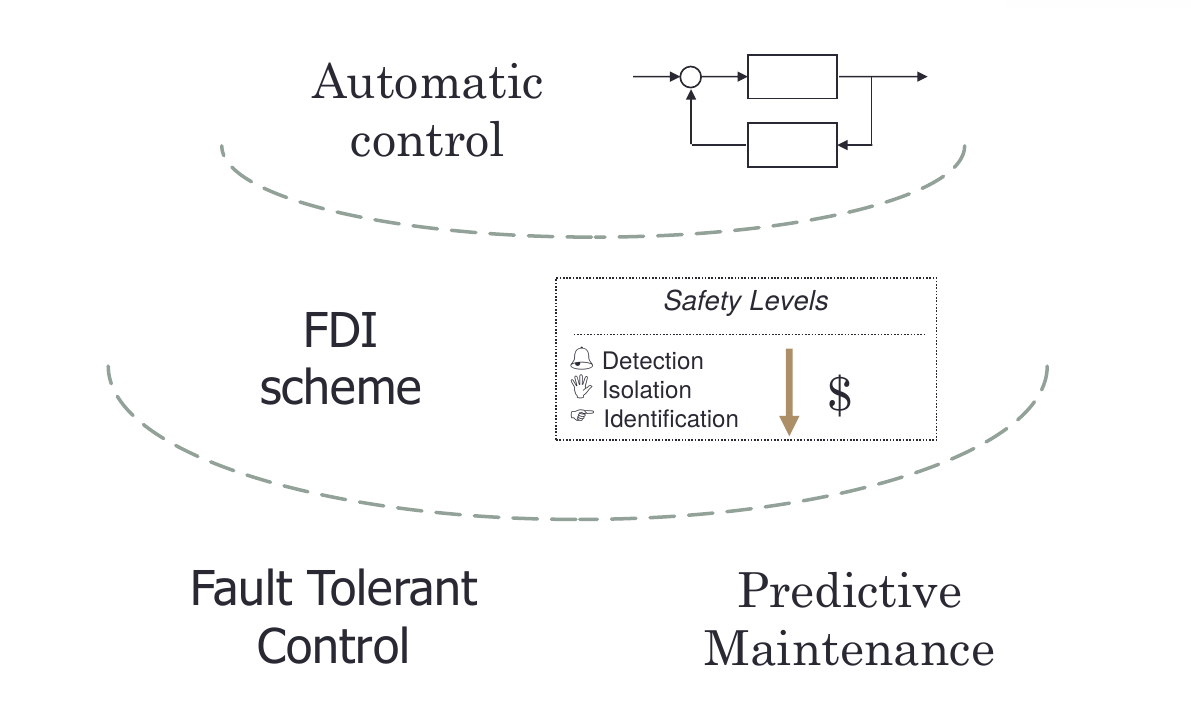
\includegraphics[scale=0.3]{FDI_PM.png}
    \caption{Relative arrangement of PdM and FDI algorithm \ref{}}
    \label{fig:fdi_pm}
\end{figure}

Figure \ref{fig:fdi_pm} presents a relative arrangement of Predictive Maintenance (PdM)
and Fault Detection and Identification (FDI or FDA) algorithms. From the
figure, it's clear that Predictive Maintenance it's an extension of the FDI
approach, with recommended workflow techniques suitable for optimizing
system maintenance. 

Both methods are closely overlapped and use quite
similar techniques. However, Predictive maintenance over the FDA is
extended by RUL estimation. And it leads not only to fault detection at a
given moment but to the possible prediction of a fault in the future. Open
the possibility of monitoring the system's state not only in the current
time but predict near-future behavior too.

\section{Applications}\label{sec:applications}
% https://www.reliableplant.com/Read/12495/preventive-predictive-maintenance

The most significant interest in PdM is the manufacturing sector that
requires efficiency maintenance strategies to increase productivity and
reduce money-lost.  Another field for PdM applications is highly dependent
on safety types of machinery such as aircraft or rail industry.  Using the
PdM condition monitoring, it's possible to prevent unexpected fails. The
oil and gas industry supports the PdM field; due to the amount of data
collected in these industries, the PdM techniques are beneficial.
